\chapter{Introduction}

The fingerprint is the systematic compilation of a certain device in order to identify it, singularize it and profile it. This data set practically allows, univocally, to identify that device and the person or group of people who may be using it. In general, devices such as mobile phones, tablets, laptops and desktop computers are used by a single person and therefore, we can assume that the data collected from a certain device belongs to a specific person. \par

Currently, web applications provide services completely free of charge in exchange for the data they collect from users. In most cases, this information is profitable through marketing and advertising services that want to sell a specific product or service. Therefore, these services need to profile the user in order to offer them a product that may interest them. Entities use these data compilation mechanisms with all devices that connect to their servers, in order to monitor the user and create a profile. \par

The best-known tracking technique are cookies, which are stored on the device and then used to study the web application's usage and to improve the user experience. It is common to find privacy clauses that allow the user to consent or not to use them. Some browsers offer the possibility of disabling their use and some antivirus perform periodic deletions of the trace files, but most web applications do not allow access to their services if the user does not allow their cookies. The use of fingerprint techniques allows not lose the traceability of the user if cookies are deleted. Technologies such as JavaScript, Flash and Microsoft Silverlight, facilitate the implementation of methods to collect very specific information about the device, such as the screen size or the operating system version. The combination of these characteristics allows the user to be profiled and identified. \par

\section{Objetives}
 

The main objective of this project is to create a web application that allows to collect data from a device, applying the different fingerprinting techniques , and to elaborate a profile based on them. Specifically, we have the following goals:
\begin{itemize}
    \item Create a scalable application, so in the future it can continue developing as required.
    \item Investigate the variety of fingerprint methods and implement them.
    \item Store the collected information, which will be outlined and saved in a database.
\end{itemize}

\section{Workplan}
For the development of the project, a plan has been established in such a way that the investigation, requirements analysis, implementation, testing and report phases are covered. \par
The figure~\ref{fig:diagramaGantten} shows the Gantt chart. After the deadlines were extended, subsequent tasks and their respective times were updated. The broken down tasks consist of:
\begin{itemize}
    \item \textbf{Investigation}: Information gathering about the existing techniques\cite{Huella} to obtain data from the devices. This includes certain pages that determine the browser's fingerprint.\cite{amiunique}.
    \item \textbf{Requirements analysis}: Assessment of what programming language and tools we are going to use for the development of the project.
    \item \textbf{Implementation}: Commissioning of the project. At this stage of development the web application would be implemented with its respective database.
    \item \textbf{Testing}: Functional check and testing of the application and resolution of possible incidents.
    \item \textbf{Report}: Document reflecting the development and results of the project.
\end{itemize}
\begin{figure}[b]
    %\centering
    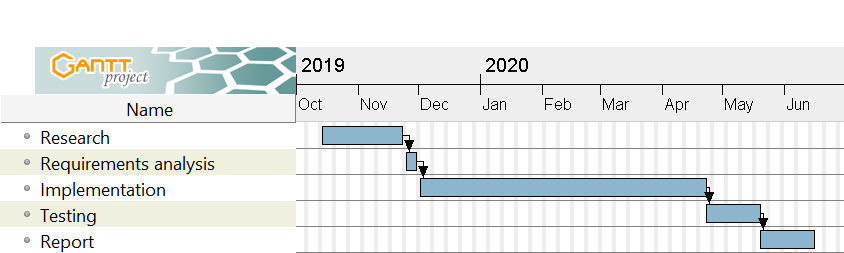
\includegraphics[width=1\textwidth, height=4cm]{Images/diagramaGantten.png}
    \caption{Gantt chart}
    \label{fig:diagramaGantten}
\end{figure}

\section{Content}
The document includes the following chapters:
\begin{itemize}
    \item \textbf{Preliminary}: Starting point and presentation of the different technologies and tools that have been explored.
    \item \textbf{Information sources}: Main data sources used for fingerprinting.
    \item \textbf{Design and implementation}: Description on how the application works.
    \item \textbf{System use}: Demonstration where the use of the application is observed.
    \item \textbf{Individual contribution}: Detailed contribution of each member of the project.
    \item \textbf{Conclusions}: Reasoned and critical discussion of the results obtained.
\end{itemize}